%%%%%%%%%%%%%%%%%%%%%%%%%%%%%%%%%%%%%%%%%
% Stylish Article
% LaTeX Template
% Version 2.1 (1/10/15)
%
% This template has been downloaded from:
% http://www.LaTeXTemplates.com
%
% Original author:
% Mathias Legrand (legrand.mathias@gmail.com) 
% With extensive modifications by:
% Vel (vel@latextemplates.com)
%
% License:
% CC BY-NC-SA 3.0 (http://creativecommons.org/licenses/by-nc-sa/3.0/)
%
%%%%%%%%%%%%%%%%%%%%%%%%%%%%%%%%%%%%%%%%%

%----------------------------------------------------------------------------------------
%	PACKAGES AND OTHER DOCUMENT CONFIGURATIONS
%----------------------------------------------------------------------------------------

\documentclass[fleqn,10pt]{SelfArx} % Document font size and equations flushed left

\usepackage[english]{babel} % Specify a different language here - english by default

%\usepackage{lipsum} % Required to insert dummy text. To be removed otherwise
%----------------------------------------------------------------------------------------
%	COLUMNS
%----------------------------------------------------------------------------------------

\setlength{\columnsep}{0.55cm} % Distance between the two columns of text
\setlength{\fboxrule}{0.75pt} % Width of the border around the abstract

%----------------------------------------------------------------------------------------
%	COLORS
%----------------------------------------------------------------------------------------

\definecolor{color1}{RGB}{0,0,90} % Color of the article title and sections
\definecolor{color2}{RGB}{0,20,20} % Color of the boxes behind the abstract and headings

%----------------------------------------------------------------------------------------
%	HYPERLINKS
%----------------------------------------------------------------------------------------

\usepackage{hyperref} % Required for hyperlinks
\hypersetup{hidelinks,colorlinks,breaklinks=true,urlcolor=color2,citecolor=color1,linkcolor=color1,bookmarksopen=false,pdftitle={Title},pdfauthor={Author}}

%----------------------------------------------------------------------------------------
%	ARTICLE INFORMATION
%----------------------------------------------------------------------------------------

\JournalInfo{Technical Report 2020-02} % Journal information
\Archive{} % Additional notes (e.g. copyright, DOI, review/research article)

\PaperTitle{Randomized Testing Strategies for Disease Spread on a Social Contact Graph} % Article title

\Authors{ Duane Currie\textsuperscript{1}*, Coleman Hooper\textsuperscript{2}, Margaret Hopkins\textsuperscript{3}, Richard Karsten\textsuperscript{3}, Yifan Li\textsuperscript{4}, Franklin Mendivil\textsuperscript{3}, Holger Teismann\textsuperscript{3}}
\affiliation{\textsuperscript{1}\textit{Institutional Research, Acadia University, Wolfville, Nova Scotia, Canada}} % Author affiliation
\affiliation{\textsuperscript{2}\textit{????}} % Author affiliation
\affiliation{\textsuperscript{3}\textit{Department of Mathematics and Statistics, Acadia University, Wolfville, Nova Scotia, Canada}} % Author affiliation%\affiliation{\textsuperscript{4}\textit{Jodrey School of Computer Science, Acadia University, Wolfville, Nova Scotia, Canada}} % Author affiliation
\affiliation{*\textbf{Corresponding author}: duane.currie@acadiau.ca } % Corresponding author


\Keywords{} % Keywords - if you don't want any simply remove all the text between the curly brackets
\newcommand{\keywordname}{Keywords} % Defines the keywords heading name

%----------------------------------------------------------------------------------------
%	ABSTRACT
%----------------------------------------------------------------------------------------

\Abstract{
The COVID-19 pandemic has highlighted the need for efficient randomized testing strategies.  Re-opening the economy, with its various consituent businesses and other organizations, includes a need for detecting outbreaks of COVID-19 before they spread to a large size.  Given that testing resources are finite, efficient strategies for randomized testing can help the re-opening process.\\[5pt]
This project explores a variety of methods to generate randomized testing schedules for an environment with known contact structures, and uses a small university as an example.\\[5pt]
\ed{Key notes about how we assessed}\\[5pt]
\ed{The results...}\\[5pt]
\ed{The conclusions...}\\[5pt]
}

\usepackage{xcolor}

\newcommand{\ed}[1]{{\color{blue} #1}}

%----------------------------------------------------------------------------------------

\begin{document}

\flushbottom % Makes all text pages the same height

\maketitle % Print the title and abstract box

\tableofcontents % Print the contents section

\thispagestyle{empty} % Removes page numbering from the first page

%----------------------------------------------------------------------------------------
%	ARTICLE CONTENTS
%----------------------------------------------------------------------------------------

\section{Introduction}

With the advent of the COVID-19 pandemic, randomized testing has come to the forefront as a strategy for managing spread of the disease.  It allows for earlier detection of cases, especially among presymptomatic and asymptomatic individuals.

Conventionally, strategies have foused on uniform random sampling.  This is true of recent university modelling as well.  However, in a university setting, there is some central knowledge of a significant portion of students' contacts, via transcript and housing data for example.  Given additional knowledge about a network of contacts, other strategies for random sampling could be employed to increase the effectiveness of the same number of individuals sampled in each round of testing.  

This paper explores a few strategies for random sampling of individuals for COVID-19 testing, and applies it to a small university setting, using representative graphs from student data at a small Canadian university.  

The methods compared are uniform random sampling, weighted sampling by total edge weight, weighted sampling by ..., sequential sampling by largest shortest path lengths, and sampling by iterative minimization of average path length to nearest sample node.  For each method, we compare the measures of expected time to noticing a first case, and expected number infected by the time a first case is known.

We also assess how these methods are impacted by reporting compliance, testing compliance, and pooled testing.

% DC:  Nothing currently for faculty and staff.  That would be a useful overlay, though.
% For faculty and staff this includes \ed{what....}


\section{Methods}

\subsection{Simulation Model}

Fundamentally, we assume knowledge of at least a significant part of the contact structure.  This has lead use to the use of agent-based modelling in a university setting, similar to choices made in other contemporary projects (cite Emory, UPenn, UCSD).  

Our simulation model uses as input graphs of interaction which signify on course co-enrolment, living in same residences, living in same residence sections, and increased likelihood of being in same locations between classes.  Each graph file contains a list of edges, along with a type identifier ("C" for course co-enrolment, "R" for living in same residence, "S" for living in same residence section, and "M" for movement between classes in same time and location), and an instance id (for example, in course co-enrolment, the instance id is a unique identifier for the specific course).  These are read into a matrix representation where the element at $(i,j)$ represents the number of the given type of interation between student $i$ and student $j$.

University life also includes students living off campus and friend-based networks.  However, these are not data that an institution may possess.  Therefore, we simulate such graphs.  Using a discrete weighted distribution of apartment sizes that students may reside in, we randomly assign students to same apartments.  We determine using the R graph which students live off campus (i.e. do not live on campus), and draw the same number of apartment sizes at random from the apartment size distribution.  We randomly resort the students and assign them in this randomized order to the available apartment spaces in order, and then truncate the list.  We then use this to build a binary adjacency matrix to represent students living in the same apartment together. Friend-based networks are generated using a Watts-Strogatz model\cite{watts_collective_1998,schnettler_structured_2009,amblard_which_2015}.  Each simulation run samples a different off-campus and friend network to incorporate into the contact structure.  

\ed{TBD:  Final contact structure as weighted sum or Poisson contact structure.}

Our disease progression is depicted in Figure~\ref{}.  Individuals begin as susceptible (S).  If they contract the disease, they become exposed (E), after which they transition to asymptomatic (A) or symptomatic (I).  If asymptomatic, they eventually recover (B).  If symptomatic, they may transition to non-infectious (J) or hospitalized (H).  From these states, they either recover (R) or die (F).  We consider them infectious in the E, I, and A states, according to a probability distribution of infectivity.  \ed{TODO:  I/A rate.  fatality rate, hospitalization rate.  transitions based on median times.}

Our simulation model initializes with all individuals susceptible, except for a given number who will begin in an exposed state.  \ed{CONSIDER: numbers per bin to initialize?  Primarily, this allows a recovered rate.}  Typically, one exposed person is used in order to simulate and measure from an index case.  

In each time step, infected individuals may infect susceptible individuals.  This is governed by determining the probability of infection per contact, which is \ed{Holger, Coleman:  details?}.  Then for each unit of contact, a draw is made to determine whether or not an infection occurs \ed{simulated using ???}.


% The transition and transmission probabilities are calibrated so that the disease dynamics generated by our model corresponds to the generally accepted transmission rates and distribution of time periods (latency period, infectious period, serial interval, etc) for COVID-19.

\subsection{Sampling Methods}

We assess several methods of sampling individuals from the graph, $G = (V,E)$, where $V$ is a set of $N$ vertices, and $E$ is a set of $K$ edges which each connect two vertices, $V_i$ and $V_j$ with weight, $w_{i,j}$.

First is a simple uniform random sample.  Here, we sample $m$ vertices from V uniformly without replacement.  This is the baseline model which is used in most prevailing studies on randomized testing for COVID-19 \ed{cite sources}.  

One may also consider those believed to interact more with others as being better candidates to sample, as they are more likely to come into contact with the disease.  For this, we implement contact weighted sampling, where each node's probability of being drawn is weighted by its total number of contacts with other nodes.  Thus, for vertex $V_i$, its weighting will be $\sum_{j \in V} w_{i,j}$.  The weights are used to form a discrete distribution, and $m$ samples are drawn from this distribution for testing.   

Another class of methods is proposed whereby the $m$ samples are drawn in such a manner as to minimize the maximum shortest path from every node to a node in the drawn set.  
In principle, the intention is to evenly spread out test subjects over the graph, taking the graph's weights into account.
In theory, this is possible to do analytically.  However, it would have the undesirable result of testing the same individuals repetitively.  Thus, we implement two methods of drawing this randomly.  

The first method is done by sequentially sampling $m$ points into a set $X$.  In the first step, a first node  that is weighted such that for vertex $i$, the weight is $\frac{1}{max_{j \in V}(sp(G, i,j))}^z$, where $sp(G,i,j)$ is the shortest path between vertices $i$ and $j$ in the graph, $G$, and $V$ is the set of vertices in $G$.  $z$ is a weighting factor - higher values of $z$ result in a higher probability of sampling from nodes with smaller maximum shortest path lengths.  In subsequent steps, the weight used for each vertex $i$ is \ed{Express it by being the value at each node, if we pick it, would be the graph's average shortest path length to the nearest node in the set}.

The second method is done in a manner motivated by self-organizing maps.  Initially, a set of $m$ vertices are chosen at random into the set $X$.  Iteratively, the node with the shortest path length to the nearest other node in $X$ is moved to the location of another drawn node by the distribution described for the first method above.  This is repeated until the improvement in average shortest path length to the nearest node in $X$ is below a provided tolerace, or until a provided maximum number of iterations is reached.

Another method is based upon graph burning \ed{cite}.  Graph burning is a means of determining how quickly all the vertices in a graph may be burned.  It is done by choosing a single node to light on fire in the first step.  Then, in each subsequent step, all nodes adjacent to a burning node are lit on fire, and another node is chosen to be lit on fire.  This procedure iterates until all nodes are on fire.  The set of nodes is the burning schedule, and the burning number for the graph is the smallest number of steps required to burn the graph.  \ed{Keep going if this seems feasible and if the node weights can be taken into account}

\subsection{Measures}

test fatigue

time to notice

cases at first notice

\subsection{Additional model parameters}

Testing delay

Testing compliance

Reporting compliance

\subsection{Procedure}

\section{Results}
\label{sec:prelimresults}


%We would describe our simulation model as being in late phases of development.  However, it can be used to illustrate the impact of some measures to manage the spread of COVID-19.  

%As a demonstration of our model, we can examine the effectiveness of masks in reducing the spread of COVID-19.  Recently, mask were documented as reducing the probability of a respiratory illess spreading between individuals by 44\%  \cite{chu_physical_2020}.  Using this in a simulation, we can observe the effect of varying degrees of mask-wearing compliance of students.  In this simulation, we assume class co-enrolment represents 3 hours/week together, passing between classes is of short duration (15 seconds), and average contact between students in a same residence is a few minutes, and between students living in a same residence section is 15 minutes longer on average.  A recent review of research suggests that 40\%-45\% of cases are asymptomatic, but that university students may be asymptomatic at a higher level \cite{oran_prevalence_2020}.  In these simulations, we assume cases have a 50\% chance of being asymptomatic.  For each level of mask compliance, 100 simulations were run with simulated off-campus living situations.  

%Figure~\ref{fig:compliance} shows the model's expected number of students infected over time, for mask compliance rates from 0\% up to 100\%.  While there is relatively little impact at low levels of mask compliance, it is clear that a high level of mask compliance (say, 80\% or above) is important to significantly flattening the curve.  It also illustrates two important points regarding mask use:  1) a high degree of mask use helps signficantly; and 2) mask use alone is not enough, and should be combined with other measures.

%\begin{figure}[ht]\centering % Using \begin{figure*} makes the figure take up the entire width of the page
%	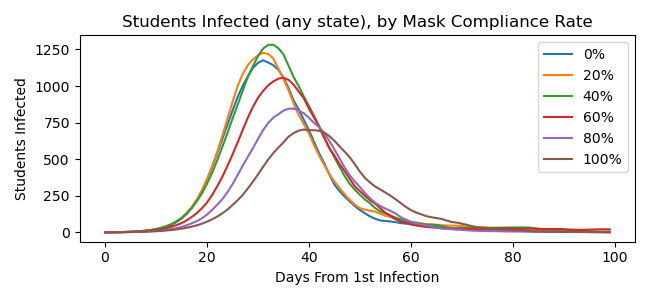
\includegraphics[width=\linewidth]{mask_compliance}
%	\caption{Effect of mask compliance on number of students infected within 100 days of first infection on campus.}
%	\label{fig:compliance}
%\end{figure}

\section{Discussion}



\section{Conclusions}


%------------------------------------------------
\phantomsection
\section*{Acknowledgments} % The \section*{} command stops section numbering
CH, MH, and YL  are funded through NSERC Discovery Grants and Acadia Professional Development funds. 

\addcontentsline{toc}{section}{Acknowledgments} % Adds this section to the table of contents


%----------------------------------------------------------------------------------------
%	REFERENCE LIST
%----------------------------------------------------------------------------------------
\phantomsection
\bibliographystyle{unsrtetal}
\bibliography{references}


%----------------------------------------------------------------------------------------

\end{document}